\chapter{Items.}
%-------------------------------------------------------------
	\section{Nombre: Peineta en forma de flor.}\label{item:peineta}
	\subsection{Descripción}
	Fue un regalo de su padre cuando niña, Malinalli la considera su mayor tesoro.
	\subsection{Imagen}
		Ver figura \ref{fig:peineta}.
		\begin{figure}
			\centering
			
\includegraphics[height=0.2 \textheight]{Imagenes/Peineta}
			\caption{Concepto peineta de Malinalli.}
			\label{fig:peineta}
		\end{figure}
	\subsection{Portador}
	Malinalli (ver apartado \ref{{per:malinalli}}).

%-------------------------------------------------------------
	\section{Nombre: Armadura espiritual.}\label{item:armadura}
	\subsection{Descripción}
	Cubre todo el cuerpo de Malinalli, pero visualmente adopta una forma que ella desee.
	\subsection{Imagen}
			Ver figura \ref{fig:armadura}.
		\begin{figure}
			\centering
			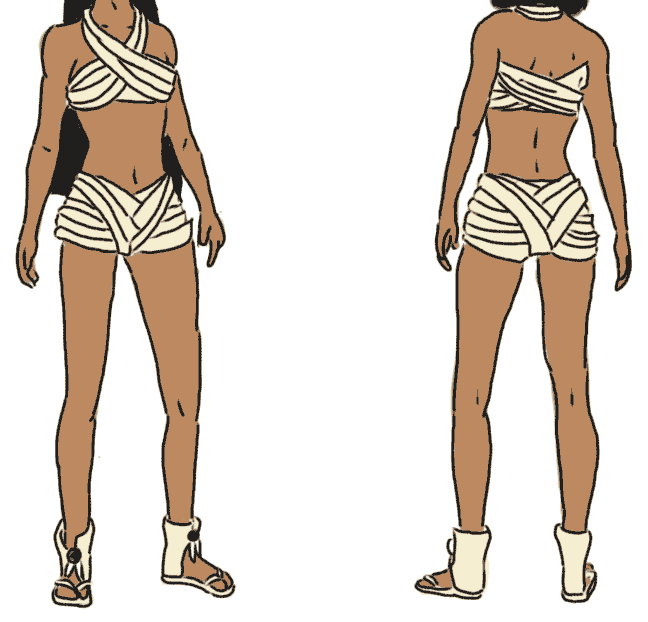
\includegraphics[height=0.2 \textheight]{Imagenes/armadura}
			\caption{Concepto armadura espiritual de Malinalli.}
			\label{fig:armadura}
		\end{figure}
	\subsection{Portador}
	Malinalli 
	
%-------------------------------------------------------------
	\section{Nombre: Flor de vainilla.}\label{item:vainilla}
	\subsection{Descripción}
	Flor de vainilla, esta rodeada de un aura dorada lo que facilita que sea vista por el jugador. Posee la capacidad de restablecer la cantidad de tonalli al hacer contacto con el jugador.
	\subsection{Imagen}
		Ver figura \ref{fig:florVainilla}.
		\begin{figure}
			\centering
			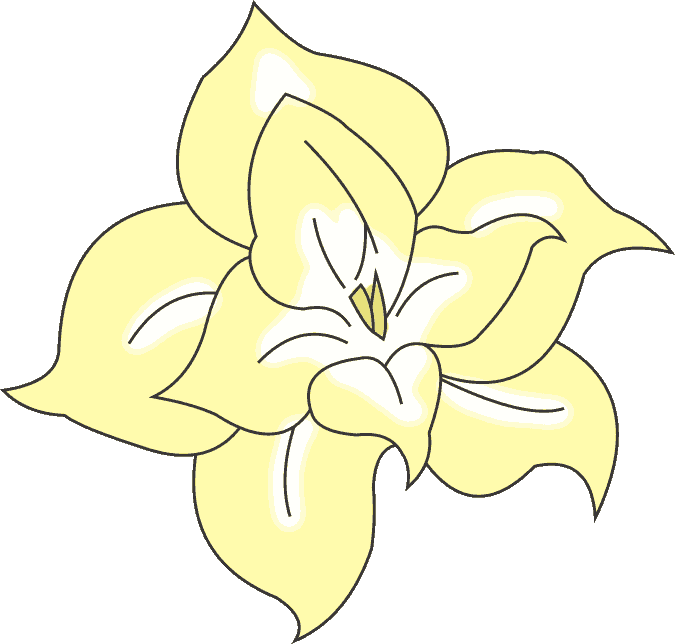
\includegraphics[height=0.2 \textheight]{Imagenes/florVainilla}
			\caption{Flor de vainilla.}
			\label{fig:florVainilla}
		\end{figure}
	\subsection{Portador}
	Malinalli 

%-------------------------------------------------------------
	\section{Nombre: Grano de cacao.}\label{item:cacao}
	\subsection{Descripción}
	Grano de cacao, esta rodeado de un aura dorada lo que facilita que sea visto por el jugador. Posee la capacidad de restablecer la cantidad de vida al hacer contacto con el jugador.
	\subsection{Imagen}
	Ver figura \ref{fig:granoCacao}.
		\begin{figure}
			\centering
			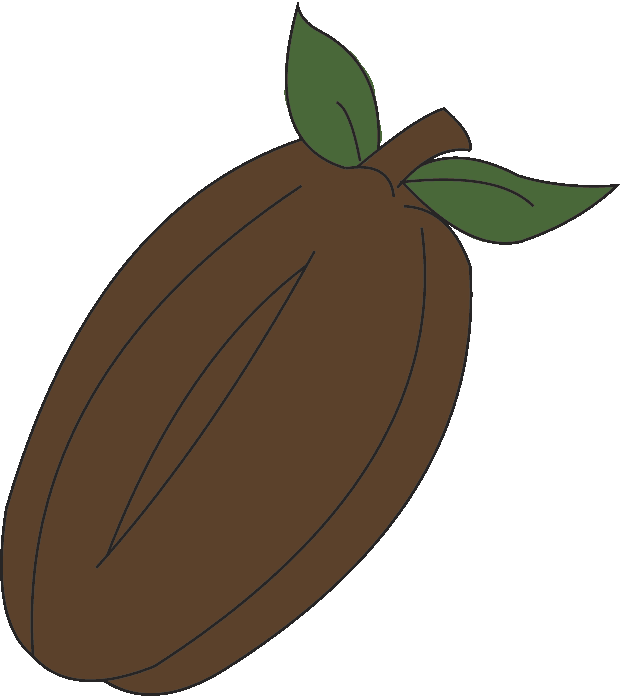
\includegraphics[height=0.2 \textheight]{Imagenes/granoCacao}
			\caption{Grano de cacao.}
			\label{fig:granoCacao}
		\end{figure}
	\subsection{Portador}
	Malinalli 

%-------------------------------------------------------------
	\section{Nombre: Xoloitzcuintle.}\label{item:Xolo}
	\subsection{Descripción}
Xoloitzcuintle de color gris. Porta un collar de oro. Se le ve nadando o acostado sobre rocas. Al hacer contacto con el jugador incrementa la cantidad de daño que puede infringir Xochitónal (ver apartado \label{Nivel:Niv02}).	
	\subsection{Imagen}
	Ver figura \ref{fig:Xoloitzcuintle}.
		\begin{figure}
  			\centering
  				\subfigure[Xoloitzcuintle acostado sobre roca.]{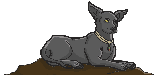
\includegraphics[width=0.45 \textwidth]{Imagenes/xolo01}}
   				\subfigure[Xoloitzcuintle nadando.]{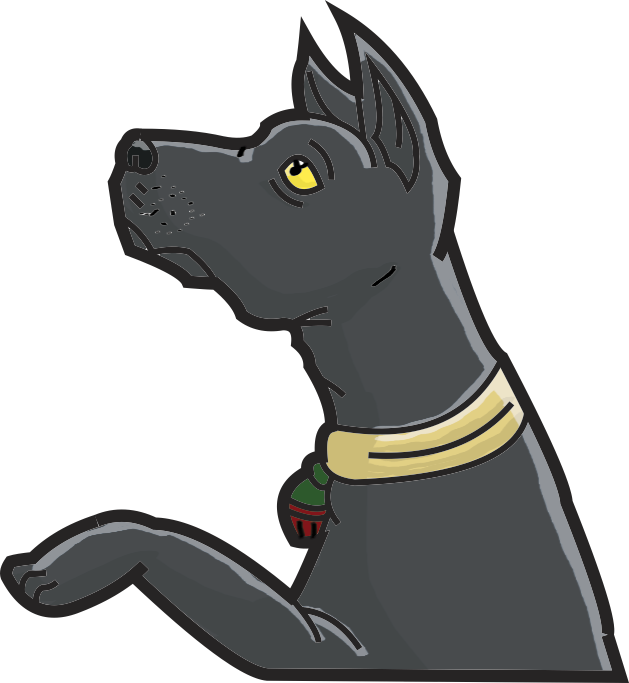
\includegraphics[width=0.2 \textwidth]{Imagenes/xolot02a}}
  				\caption{Conceptos de diseño de Xólotl.}
  			\label{fig:Xoloitzcuintle}
		\end{figure} 
		
	\subsection{Portador}
	Sin portador. 

%-------------------------------------------------------------
	\section{Mariposa} \label{item:Mariposa}
		\subsection{Descripción}
		Mariposa azul de tamaño normal. Se encontrara en diferentes puntos del mapa del nivel 4 (ver apartado \ref{Nivel:Niv04})  para indicarle al jugador que esta siguiendo el camino correcto al templo de Itzpapálotl.
		\subsection{Imagen}
		Ver figura \ref{fig:Mariposa}.
		\begin{figure}
			\centering
			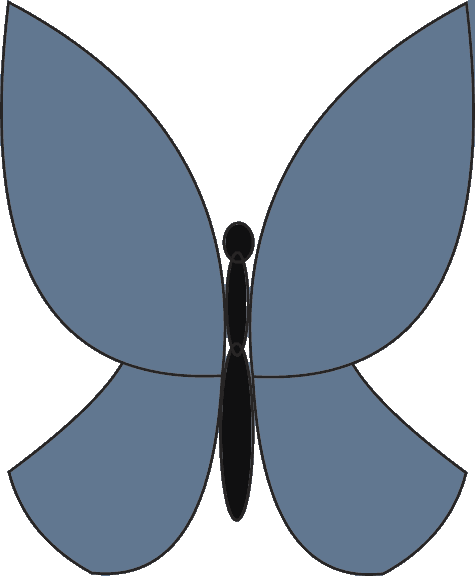
\includegraphics[height=0.2 \textheight]{Imagenes/mariposa}
			\caption{Mariposa.}
			\label{fig:Mariposa}
		\end{figure}
	\subsection{Portador}
	Sin portador. 
	
%---------------------------------------------------------------
\section{Llave de la guarida de Itzpápalotl} \label{item:LlaveItz}
		\subsection{Descripción}
		
Llave que permite abrir la entrada a la guarida de Itzpápalotl. En total son tres y están custodiadas por diferentes enemigos (ver apartado \ref{Nivel:Niv04}).
		\subsection{Imagen}
		Ver figura \ref{fig:llaveMariposa}.
		\begin{figure}
			\centering
			
\includegraphics[height=0.2 \textheight]{Imagenes/items}
			\caption{Llave de la guarida de Itzpápalotl.}
			\label{fig:llaveMariposa}
		\end{figure}
	\subsection{Portador}
	Sin portador. 